%----------------------------------------------------------------------------------------
%	PACKAGES AND OTHER DOCUMENT CONFIGURATIONS
%----------------------------------------------------------------------------------------

\documentclass[12pt]{article}
\usepackage{graphicx}
\usepackage[utf8]{inputenc}  
\usepackage[T1]{fontenc} 
\usepackage[top=1.5cm,bottom=1.5cm,left=1.3cm,right=1cm,asymmetric]{geometry}

\usepackage{amsfonts}
\usepackage{graphicx}
\usepackage{amsmath}
\usepackage{fancyhdr}
\usepackage{array,multirow,makecell}
\usepackage{cancel}
\usepackage{subfig}
\usepackage{wrapfig}
\setcellgapes{1pt}
\makegapedcells
\newcolumntype{R}[1]{>{\raggedleft\arraybackslash }b{#1}}
\newcolumntype{L}[1]{>{\raggedright\arraybackslash }b{#1}}
\newcolumntype{C}[1]{>{\centering\arraybackslash }b{#1}}


\usepackage{tikz}
\usetikzlibrary{arrows,automata,fit}

\pagestyle{fancy}
\renewcommand{\footrulewidth}{1pt}
\fancyhead[R]{\textit{Master MVA : Probabilistic graphical models}}
\fancyfoot[L]{\textit{}}
%\usepackage{unicode-math}
%\setmathfont{XITS Math}
%\setmathfont[version=setB,StylisticSet=1]{XITS Math}


%\geometry{hmargin=1.5cm,vmargin=2cm}   

\begin{document}
\section*{Latent dirichlet allocation for label modelling}
\section*{Thibaud Ehret \& Sammy Khalife}
~\\
\section*{Presentation of the model [Journal of Machine Learning, 2003]}
\begin{figure}[!H]
	\centering
	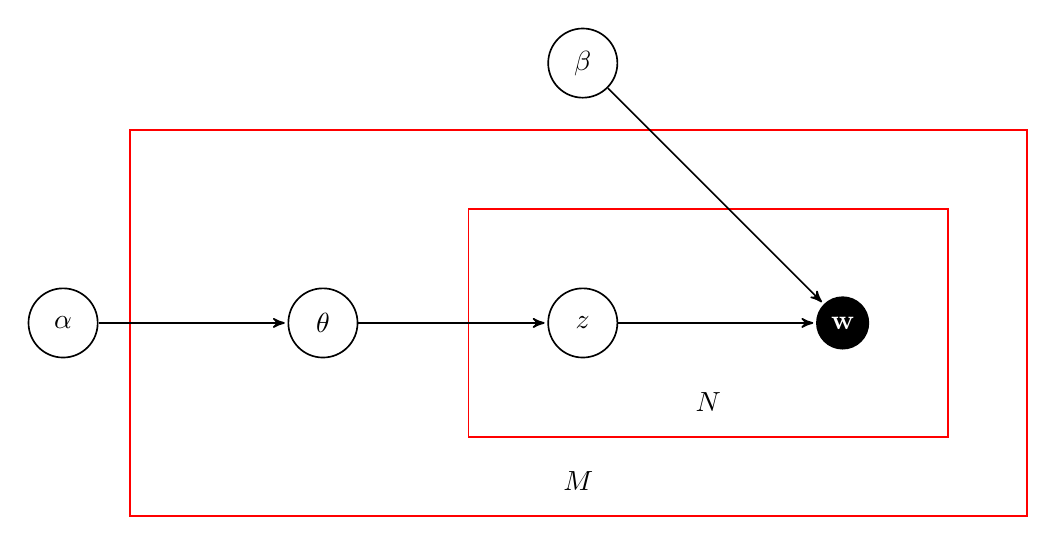
\begin{tikzpicture}[->,>=stealth',shorten >=1pt,auto,node distance=3.3cm,
		semithick]
		\tikzstyle{every state}=[fill=white,draw=black,text=black]
		\tikzstyle{final}=[circle, fill=black,draw=black,text=white]
		\node[state]         (A)                    {$\alpha$};
		\node[state]         (B) [right of=A]       {$\theta$};
		\node[state]         (C) [right of=B]       {$z$};
		\node[state]         (D) [above of=C]       {$\beta$};
		\node[final]         (E) [right of=C]       {$\textbf{w}$};
		\node (B1) [draw=red, fit= (E) (B) (C) , inner sep=2cm] {};
		\node (B2) [draw=red, fit= (C) (E), inner sep=1cm] {};
		\node [yshift=3.0ex, black] at (B1.south) {$M$};
		\node [yshift=3.0ex, black] at (B2.south) {$N$};
		\path (A) edge              (B)
	              (C) edge              (E)
	              (D) edge              (E)
	              (B) edge              (C);
	\end{tikzpicture}
	\caption{LDA model}
	\label{LDA_model}
\end{figure}

~\\
In the latent dirichlet model (LDA), there are different levels of representation of the object concerned (documents in our case). It differs from a simple multinomial model in the sense that each object can be associated with multiple topics. ~\\
~\\
\textbf{Generation of documents}~\\
~\\
The parameter $\theta$  which belongs to $\mathbb{R}^{d}$ is sampled once per document from a smooth distribution on the topic simplex, and represents the distribution of the topics within the document. $\theta$ is generated through a dirichlet distribution of parameter $\alpha$. We suppose that each word $\textbf{w}$ is generated through a multinomial probability conditionned on the topic : $\beta \in \mathbb{R}^{K*V}$, with $\beta_{ij}=p(w^{j}=1|z^{i}=1)$, V representing the number of possible words, and K the number of topics.

\begin{eqnarray*}
p(\textbf{w}|\alpha, \beta) &  = & \int p(\theta | \alpha, \beta)p(\textbf{w} | \alpha, \beta, \theta)d\theta\\
\end{eqnarray*}
In the LDA model, we have $ \theta \perp \beta$, and $p(w_{i} | \alpha, \beta, \theta) \perp p(w_{j} | \alpha, \beta, \theta)$  for $ i \neq j $
\begin{eqnarray*}
p(\textbf{w}|\alpha, \beta) & = & \int p(\theta | \alpha) \prod_{n=1}^{N} p(\textbf{w}_{n} | \alpha, \beta, \theta)d\theta\\
& = & \int  p(\theta |\alpha) \prod_{n=1}^{N}  \sum_{z_{n}}p(z_{n}|\alpha, \beta, \theta)p(\textbf{w}_{n} | \alpha, \beta, \theta, z_{n}) d\theta\\
\end{eqnarray*}
Moreover $z \perp (\alpha,\beta)$ and $\textbf{w}_{n} \perp (\alpha,\theta)$, then
\begin{eqnarray*}
p(\textbf{w}|\alpha, \beta) & = & \int p(\theta | \alpha)  \prod_{n=1}^{N}  \sum_{z_{n}}p(z_{n} |\theta)p(\textbf{w}_{n} | z_{n}, \beta) d\theta\\
\end{eqnarray*}

\section*{Inference and parameter estimation}
Then the natural inferential problem that we need to solve in order to use LDA, is to compute :
$$p(\theta, \textbf{z}|\textbf{w},\alpha,\beta)=\frac{p(\theta,\textbf{z},\textbf{w}|\alpha,\beta)}{p(\textbf{w}|\alpha,\beta)}$$
Unfortunately, this expression is intractable due to the coupling between $\theta$ and $\beta$.
Then, an EM scheme is used to make an inference on parameters $\alpha$ and $\beta$. ~\\

\section{The algorithm}
We saw the complexity of the distribution associated to this model, therefore one can not simply calculate the posterior distribution for the inference and the parameter estimation. We will briefly present the algorithm used to calculate the inference and an approximation of the parameters. However, even if the distribution can not be computed, the algorithm is based on the EM principle.

\subsection{Inference}

The trick to be able to calculate the inference for the LDA model to calculate the variational inference which is a lower bound but easily calculable.

The lower bound is computed using the simplified graphical model presented in figure \ref{low_bound_model} which does not have the coupling between $\theta$ and $\beta$ and $\textbf{w}$.

The parameters $\gamma$ and $\phi$ for this new model are estimated by minimmizing the Kullback-Leibler divergence which has been shown to be good lower bound for the log-likelyhood. These are the parameters that we will use in the next part in order to estimate the parameters. 

\subsection{Parameter estimation}

We uses a modified version of the EM algorithm for this part. The expectation part, also called E-step, consists in computed the best variational parameters $\gamma$ and $\phi$ for the lower bound presented in the previous section. The maximization part, M-step, consists in optimizing the model parameter $\alpha$ and $\beta$ with the variational parameter fixed.
Just like in the EM algorithm, both step are then iterated until the bound of the model \ref{low_bound_model} converges.

\begin{figure}
	\centering
	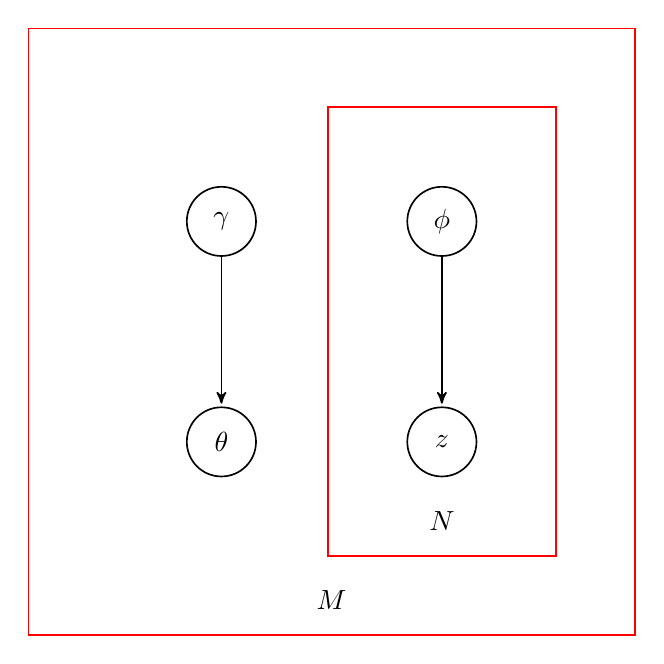
\begin{tikzpicture}[->,>=stealth',shorten >=1pt,auto,node distance=2.8cm,
		semithick]
		\tikzstyle{every state}=[fill=white,draw=black,text=black]
		\node[state]         (A)                    {$\gamma$};
		\node [state]        (B) [below of=A]       {$\theta$};
		\node[state]         (C) [right of=A]       {$\phi$};
		\node[state]         (D) [below of=C]       {$z$};
		\node (B1) [draw=red, fit= (A) (B) (C) (D), inner sep=2cm] {};
		\node (B2) [draw=red, fit= (D) (C), inner sep=1cm] {};
		\node [yshift=3.0ex, black] at (B1.south) {$M$};
		\node [yshift=3.0ex, black] at (B2.south) {$N$};
		\path (A) edge              (B)
	              (C) edge              (D);
	\end{tikzpicture}
	\caption{Graphical model used to calculate the lower bound of the log-likelyhood for the LDA graphical model}
	\label{low_bound_model}
\end{figure}

\section{Experiments}
We tried the model on 2 toy examples, one made with 4 documents containing the same word and having a different word per document, and the second example with 4documents, 2 of them having a the same words in them.

For the first dataset depending on the initialisation, we can find a topic per word which correspond to what we could have expected or 2 words can be wrongfully associated in the same topic. That shows the limitations of using so many approximtions during the procedures.

For the second dataset the two topic found are the one that could have been expected , the words that are in the same document are said to be in the same topic.

\end{document}
